\section{Evaluation}
\label{sec:cfa:eval}


In this section, we show that:
\begin{packeditemize}
\item \dda  predicts video quality with 30\% less error than 
competing machine learning algorithms 
(Section~\ref{subsec:eval-accuracy}).
\item Using \dda-based prediction, we can improve  
video quality significantly; e.g., 32\% less BufRatio, 
12\% higher AvgBitrate in a pilot deployment 
(Section~\ref{subsec:eval-improvement}).
% than those selected by a baseline players. 
%More extensive trace-driven simulation shows that across different quality metrics, \dda leads to 5-17\% improvement over decisions made by the more accurate prediction algorithms other than \dda.
\item \dda is responsive to client  queries and  makes 
predictions based on the most recent critical features 
and quality measurements 
(Section~\ref{subsec:eval-scalability}).
\end{packeditemize}


%\begin{figure*}[t!]
%\centering
%\hspace{-0.5cm}
%\subfigure[Distribution of per-session prediction error]
%{
%        \includegraphics[width=0.5\textwidth]{eval-figs/batch-3/barchart-distribution.pdf}
%        \label{subfig:per-session-error}
%}
%\hspace{-0.3cm}
%\subfigure[Kendall rank correlation coefficient]
%{
%         \includegraphics[width=0.5\textwidth]{eval-figs/batch-3/barchart-correlation.pdf}
%        \label{subfig:kendall}
%}
%\hspace{-0.5cm}
%\vspace{-0.3cm}
%\tightcaption{Compared with conventional machine learning techniques (green) and naive prediction algorithms (blue), \dda can accurately predict each session's quality and the rank between different quality values (Kendall coefficient).}
%\vspace{-0.3cm}
%\label{fig:accuracy}
%\end{figure*}


\begin{figure}[t!]
\centering
%\hspace{-0.6cm}
\subfloat[AvgBitrate]
{
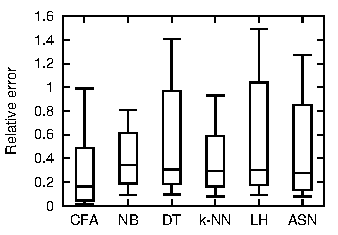
\includegraphics[width=.4\textwidth]{figures/cfa-barchart-distribution-AvgBitrate.pdf}
        \label{subfig:accuracy-avgbitrate}
}
%\hspace{-0.4cm}
\subfloat[JoinTime]
{
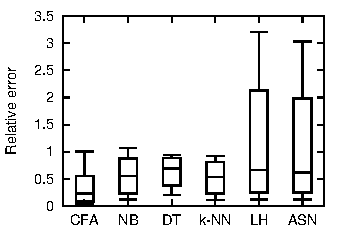
\includegraphics[width=.4\textwidth]{figures/cfa-barchart-distribution-JoinTime.pdf}
        \label{subfig:accuracy-avgbitrate}
}
%\hspace{-0.6cm}
\\
%\vspace{-0.25cm}
%\hspace{-1cm}
\subfloat[BufRatio]
{
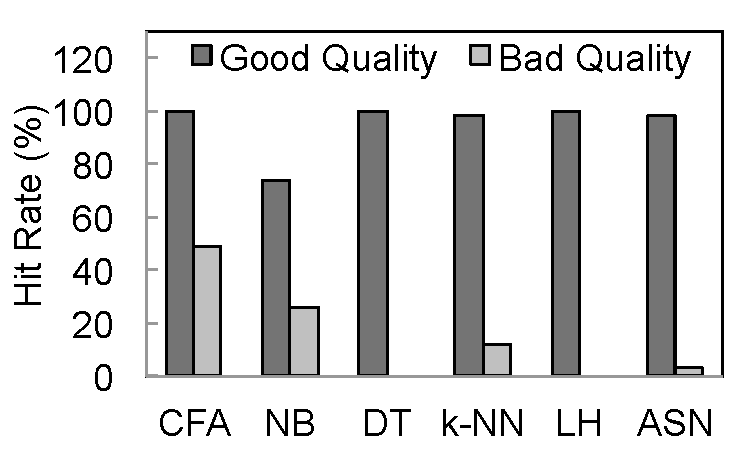
\includegraphics[width=.4\textwidth]{figures/cfa-HitRate-BufRatio.pdf}
        \label{subfig:accuracy-bufratio}
}
%\hspace{-0.4cm}
\subfloat[VSF]
{
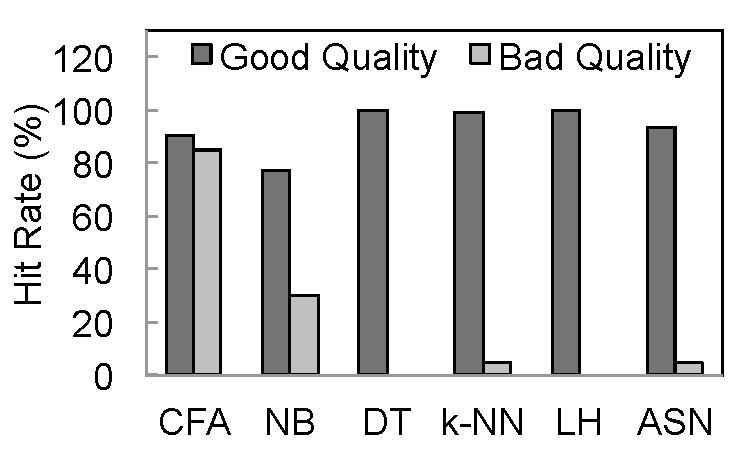
\includegraphics[width=.4\textwidth]{figures/cfa-HitRate-VSF.pdf}
        \label{subfig:accuracy-vsf}
}
\caption{Distributions of relative prediction error ($\{5,10,50,90,95\}\%$iles) on AvgBitrate and JoinTime and hit rates on BufRatio and VSF. They show that \dda outperforms other algorithms.}
%\vspace{-0.3cm}
\label{fig:accuracy}
\end{figure}

\subsection{Prediction Accuracy}
\label{subsec:eval-accuracy}
We compare \dda with five alternative algorithms: three
simple ML algorithms, Naive Bayes (NB), Decision Tree (DT),
$k$-Nearest Neighbor ($k$-NN)\footnote{NB, DT, and 
$k$-NN are mplemented using a popular ML
library \texttt{weka}\cite{weka}.}, and two heuristics 
 which predict a session's quality by the average quality 
of other sessions from the same ASN (ASN) or matching 
the last-mile connection type (LH). 
All algorithms use the same set of features listed in 
Table~\ref{tab:features}.


%First, we show that \dda yields high prediction accuracy. 

Ideally, we want to evaluate how accurately an algorithm 
can predict the quality of a given client on every choice 
of CDN and bitrate. 
However,  this is infeasible since each video client is 
assigned to only one CDN and bitrate at any time.
Thus,  we  can only evaluate the prediction accuracy 
over the observed CDN-bitrate choices, and we use the 
quality measured on these choices as the ground truth.
%A caveat of this methodology is that it evaluates the accuracy only over decisions of bitrate and CDN that were actually made.%; i.e., the error is not over the entire space of decisions. 
That said, this approach is still useful for doing a relative 
comparison across different algorithms.  

%\myparatight{Per-session prediction error} 
For AvgBitrate and JoinTime, we report {\em relative error}:
$\frac{|p-q|}{q}$, where the $q$ is the ground truth and 
$p$ is the prediction.
For  BufRatio and JoinTime, which have more ``step 
function'' like effects~\cite{sigcomm11}, we report a 
slightly different measure called {\em hit rate}:
how likely a session with good quality (i.e., 
BufRatio~$<5\%$, VSF=0) or bad quality is correctly 
identified. 
%We compare the prediction accuracy over 20 millions sessions from a real dataset of a week.
Figure~\ref{fig:accuracy} shows that for AvgBitrate and
JoinTime, \dda has the lowest $\{5,10,50,90\}\%$th 
percentiles of prediction error and lower $95\%$th 
percentiles than most algorithms.  
In particular, median error of \dda is about 30\% lower 
than the best competing  algorithm.  
In terms of BufRatio and VSF, \dda significantly 
outperforms other algorithms in the hit rate of bad 
quality sessions. 
The reason  for hit rate of bad quality to be lower than 
that of good quality is that bad quality sessions are 
almost always less than good quality, which makes 
them hard to predict.
Note that accurately identifying sessions that have bad 
quality is crucial as they have the most room for 
improvement.


%\myparatight{Rank correlation} In addition to prediction error, it is also useful to quantify whether the prediction algorithm can accurately identify the {\em rank} of two quality values. To this end, we calculate the Kendall rank correlation coefficient between actual and predicted quality of different algorithms. 
%%To ensure the rank is meaningful, we exclude duplicated actual quality. 
%Figure~\ref{subfig:kendall} shows that \dda has much higher Kendall rank correlation coefficient than the five strawman algorithms, which means \dda can better differentiate different quality values.
%An interesting observation is that \dda has more advantages on BufRatio and VSF, where \dda does not have much better prediction error in Figure~\ref{subfig:per-session-error}. This is because most values of BufRatio and VSF are zero (i.e., no extra buffering or no start failure). While most algorithms can easily achieve low error on these zero values, it is hard for them to predict other values accurately.



\subsection{Quality Improvement}
\label{subsec:eval-improvement}

%Next, we show that CDN and bitrate selected based on quality prediction of \dda leads to better quality than baseline approaches. We show it by a real-world pilot deployment as well as real-world trace-driven simulation.


\mypara{Pilot deployment}
As a pilot deployment, we integrated \dda in a production 
system that provides a global video optimization 
service~\cite{c3}.
% that manages delivery for several premium band content providers.  
We deployed \dda on one major content provider and used it 
 to optimize 150,000 sessions each day.
% by selecting among 3 CDNs and 6 bitrates.
%To demonstrate the improvement using \dda, 
We ran an A/B test (where each algorithm was used on 
a random subset of clients) to  evaluate the improvement 
of \dda over a baseline random decision maker, which 
many video optimization services  use by default (modulo 
business arrangement like price)~\cite{hulu}.
%\footnote{\dda is also better than the custom  algorithm 
% used in production. Due to proprietary concerns, we do not show quantitative results vs.\  production strategies.
%\camera{Qualitatively, \dda is automated while the custom algorithm has had several rounds of manual tweaking, so the fact that \dda is better is already promising. Furthermore, conversations with engineers were positive, and they were willing to invest time in implementing \dda and running longer pilots.}  }



\begin{table}[t!]
\begin{center}
%\begin{small}
\begin{tabular}{l|c|c|c}
 & \dda & Baseline & Improvement \\ \hline \hline
QoE & 155.43 & 138.27 & 12.4\% \\
BufRatio & 0.0123 & 0.0182 & 32\% \\ 
AvgBitrate & 3200 & 2849 & 12.31\% \\
\end{tabular}
%\end{small}
%\vspace{-0.2cm}
\caption{Random A/B testing results of \dda vs. baseline in 
real-world deployment.}
%\vspace{-0.2cm}
%\vspace{-0.4cm}
\label{tab:pilot-statistics}
\end{center}
\end{table}


\begin{figure*}[t!]
\centering
\subfloat[\dda vs.\ baseline by time]
{
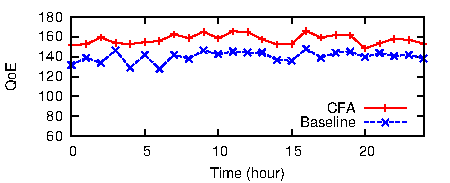
\includegraphics[width=.6\textwidth]{figures/cfa-realimp-timeseries--1.pdf}
        \label{subfig:per-session-error}
}\\
%\hspace{-0.8cm}
\subfloat[\dda vs.\ baseline by spatial partitions]
{
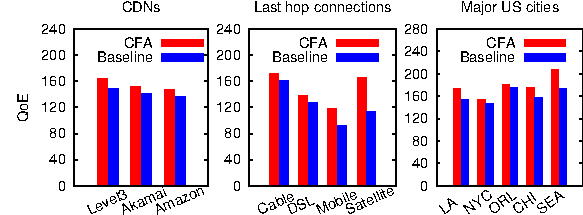
\includegraphics[width=.8\textwidth]{figures/cfa-realimp-bar-partitions--1.pdf}
        \label{subfig:real-world-spatial}
}
%\vspace{-0.3cm}
\caption{Results of real-world deployment. 
\dda outperforms the baseline random decision maker 
(over time and across different large cities, connection t
ypes and CDNs).}
%\vspace{-0.4cm}
\label{fig:real-world-improvement}
\end{figure*}


Table~\ref{tab:pilot-statistics} compares \dda with the 
baseline random decision maker in terms of the mean 
BufRatio, AvgBitrate
%\footnote{JoinTime and VSF are not shown as they are not explicitly optimized} 
and a simple QoE model 
($QoE=-370*BufRatio+AvgBitrate/20$), which was 
suggested by~\cite{sigcomm12,sigcomm11}. 
Over all sessions in the A/B testing, \dda shows an 
improvement in both BufRatio (32\% reduction) and 
AvgBitrate (12.3\% increase) compared to the baseline.
This shows that \dda is able to simultaneously optimize
multiple (possibly conflicting) metrics. 
To put these numbers in context, our conversation 
with domain experts  confirmed that these 
improvements are significant for content providers and 
 can potentially translate into  substantial benefits in 
 engagement and revenues~\cite{convivapersonal}.
% \dda's superior performance and our conversations with domain experts indicate that they were willing to invest time running longer pilot.
\dda's superior performance and that  \dda is more 
automated than the custom algorithm indicate that 
domain experts were willing to invest time running 
longer pilot.
Figure~\ref{fig:real-world-improvement} provides 
more comparison and shows that \dda consistently 
outperforms the baseline over time and across different 
major cities in the US, connection types and CDNs. 
%Especially, quality of each CDN is improved, which means quality can be 
%improved by only selecting bitrate based on \dda prediction.


%\vyas{where are the numbers in 6.0 coming from??}


\mypara{Trace-driven simulation}
%While real-world deployment is realistic, it has inherent constraints such as load of CDNs (e.g., in the pilot deployment, the traffic assigned to each CDN needs to be within a lower and upper bound due to business contract), and limited scalability to simultaneously evaluate many instantiations of prediction systems. 
%Trace-driven evaluation may address these constraints, but it needs to estimate the quality of decisions that had not been used. 
We complement this real-world deployment with a 
trace-driven simulation to simultaneously compare 
more algorithms over more quality metrics. 
However, one key challenge is that it is hard to 
estimate the quality of a decision that was not used 
by a specific client in the trace.

To address this problem, we use the 
{\em counterfactual methodology} from prior work in 
online recommendation 
systems~\cite{li2010contextual,li2011unbiased}.
Suppose we have quality measurements from a 
set of clients,
where client $c$ is assigned to a decision $d_{rand}(c)$ 
of CDN and bitrate at random.
Now, we have a new hypothetical algorithm that maps 
client $c$ to $d_{alg}(c)$. 
Then, we can evaluate the average quality of clients 
assigned to each decision $d$,  $\{c|d_{alg}(c)=d\}$, 
by the average quality of $\{c|d_{alg}(c)=d,d_{rand}(c)=d\}$.
Finally, the average quality of the new algorithm is 
the weighted sum of average quality of all decisions, 
where the weight of each decision is the fraction of 
sessions assigned to it.
% being randomly assigned to a decision (CDN and bitrate).
%Then, to evaluate a different assignment between the same clients and decisions, 
%we can estimate the average quality of each decision in the 
%new assignment by the average quality of the clients that are assigned 
%to this decision in both new assignment and the previous random assignment.
This can be proved to be an unbiased (offline) 
estimate of $d_{alg}$'s (online) 
performance~\cite{austin2011introduction}.\footnote{One known 
limitation of this analysis is that it assumes the new 
assignments do not affect each decision's overall 
performance. 
For instance, if we assign all sessions to one CDN, 
they may overload the CDN and so this CDN's quality 
in the random assignments is no longer useful. 
Since this work only focuses on controlling traffic at a 
small scale relative to the total load on the CDN (and 
our experiments are in fact performed at such a scale), 
this methodology is still unbiased.}
For instance, if out of 1000 clients assigned to use 
Akamai and 500Kbps, 200 clients are assigned to this 
decision in the random assignment, then we can use 
the average quality of these 200 sessions as an unbiased
estimate of the average quality of these 1000 sessions.
%for each decision (i.e., a specific CDN and bitrate), we first randomly select a subset of client to use the decision (i.e., the selection is independent to any aspect of a client). Then, given a new assignment of the same clients, for each decision, the subset of client that are assigned to this decision in both random assignment and new assignment represents an unbiased estimation of average quality of this decision in the new assignment. 
%It can be proved to be an {\em unbiased} estimate of average quality of 
%any new decision assignment\footnote{}.
%For a proof, please refer~\cite{cfe-report}.
Fortunately, our dataset includes a (randomly chosen) 
portion of clients with randomized decision assignments 
(i.e., CDN and bitrate). 
Thus, we  only report improvements  for these clients. 
 %such content providers and restrict the evaluation  to these clients.



\begin{figure}[t!]
\centering
%\hspace{-0.4cm}
%\subfigure[QoE]
%{
%\includegraphics[width=.2\textwidth]{eval-figs/batch-3/cfImp--1.pdf}
%        \label{subfig:Imp-cfImp--1}
%}
%\hspace{-0.4cm}
%\subfigure[BufRatio]
%{
%\includegraphics[width=.2\textwidth]{eval-figs/batch-3/cfImp-0.pdf}
%        \label{subfig:Imp-cfImp-0}
%}
%\hspace{-0.4cm}
%\subfigure[AvgBitrate]
%{
%\includegraphics[width=.2\textwidth]{eval-figs/batch-3/cfImp-1.pdf}
%        \label{subfig:Imp-cfImp-1}
%}
%\hspace{-0.4cm}
%\subfigure[JoinTime]
%{
%\includegraphics[width=.2\textwidth]{eval-figs/batch-3/cfImp-2.pdf}
%        \label{subfig:Imp-cfImp-2}
%}
%\hspace{-0.4cm}
%\subfigure[VSF]
%{
%\includegraphics[width=.2\textwidth]{eval-figs/batch-3/cfImp-3.pdf}
%        \label{subfig:Imp-cfImp-3}
%}
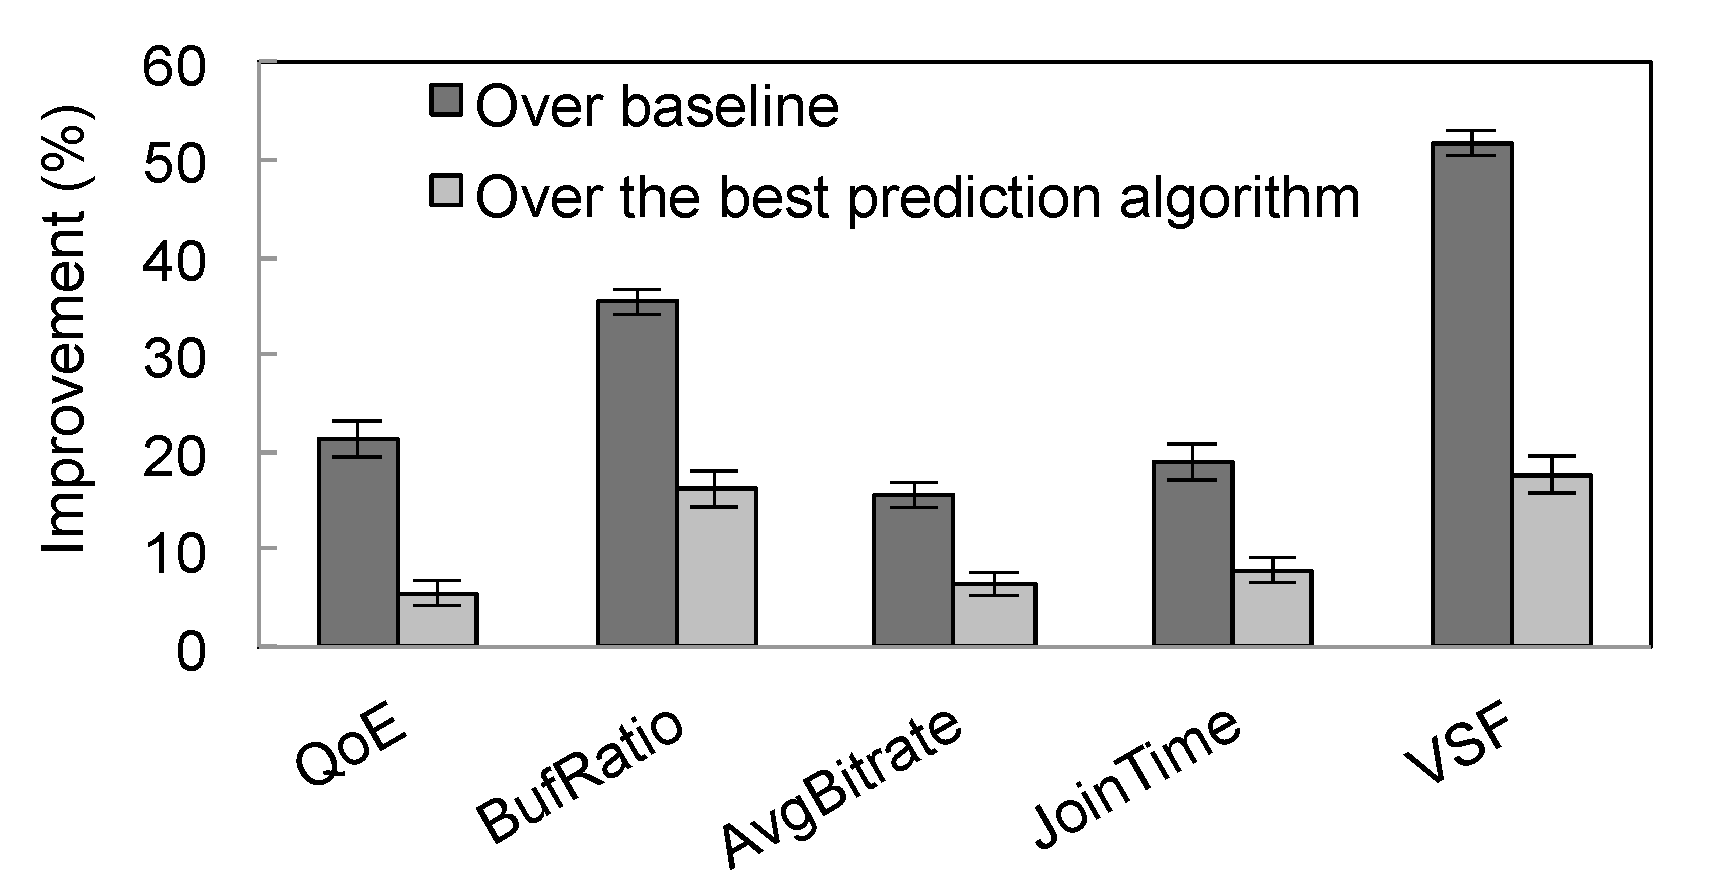
\includegraphics[width=0.6\textwidth]{figures/cfa-CF-IMPROVEMENT-Perc-Grouped.pdf}
%\vspace{-0.3cm}
\caption{Comparison of quality improvement 
between \dda and strawmen.}
%\vspace{-0.3cm}
\label{fig:trace-driven-improvement}
\end{figure}


Figure~\ref{fig:trace-driven-improvement} uses this 
counterfactual methodology and compares \dda with the 
best alternative from Section~\ref{subsec:eval-accuracy} for 
each quality metric and the baseline random decision 
maker (e.g., the best alternative of AvgBitrate is k-NN). 
For each quality metric and prediction algorithm, the 
decision maker selects the CDN and bitrate that has 
the  best predicted quality for each client. 
For instance, the improvement of \dda over the baseline 
on VSF is 52\% -- this means the number of sessions 
with start failures is 52\% less than when the baseline 
algorithm is used.
The figures show that \dda outperforms the baseline 
algorithm by 15\%-52\%. 
They also show that \dda outperforms the best prediction 
algorithms by 5\%-17\%. %\vyas{make numbers consistent with 6.0 and intro}



\subsection{Timeliness of Prediction}
\label{subsec:eval-scalability}

Our implementation of \dda should
(1) retain freshness to minimize the impact of staleness on prediction accuracy, and 
(2) be responsive to each prediction query. 




\begin{figure}[t!]
\centering
%\hspace{-0.6cm}
\subfloat[BufRatio]
{
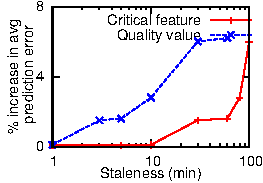
\includegraphics[width=.36\textwidth]{figures/cfa-insight-staleness-impact-0.pdf}
        \label{subfig:Imp-cfImp--1}
}
%\hspace{-0.4cm}
\subfloat[AvgBitrate]
{
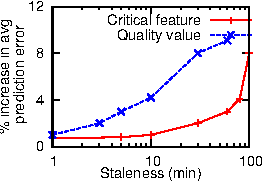
\includegraphics[width=.36\textwidth]{figures/cfa-insight-staleness-impact-1.pdf}
        \label{subfig:Imp-cfImp-0}
}
%\hspace{-0.6cm}
\\
%\vspace{-0.2cm}
%\hspace{-1cm}
\subfloat[JoinTime]
{
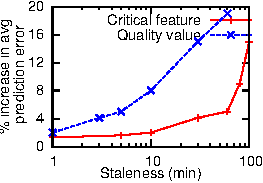
\includegraphics[width=.36\textwidth]{figures/cfa-insight-staleness-impact-2.pdf}
        \label{subfig:Imp-cfImp-1}
}
%\hspace{-0.4cm}
\subfloat[VSF]
{
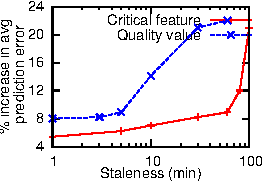
\includegraphics[width=.36\textwidth]{figures/cfa-insight-staleness-impact-3.pdf}
        \label{subfig:Imp-cfImp-2}
}
%\hspace{-0.6cm}
%\vspace{-0.3cm}
\caption{Latency of critical features and quality values 
(x-axis) on increase in accuracy (y-axis).}
%\vspace{-0.2cm}
\label{fig:insight-staleness}
\end{figure}


\begin{table}[t!]
\begin{center}
%\begin{small}
\begin{tabular}{p{2in}|p{2in}|p{2in}}
{\bf Stage} & {\bf Run time (mean / median)} & {\bf Required freshness} \\ \hline \hline
Critical feature learning & 30.1/29.5 min & 30-60 min \\
Quality estimation  &  30.7/28.5 sec & 1-5 min \\
Query response	 &  0.66/0.62 ms & 1 ms
\end{tabular}
%\end{small}
\caption{Each stage of \dda is refreshed to meet the 
required freshness of its results.}
\label{tab:response-all}
\end{center}
%\vspace{-0.7cm}
\end{table}


We begin by showing how fast each stage described 
in Section~\ref{subsec:scalability} needs to be refreshed. 
Figure~\ref{fig:insight-staleness} shows the impact of 
staleness of critical features and quality values on the 
prediction accuracy of \dda. 
First, critical features learned 30-60 minutes before 
prediction can still achieve similar accuracy as those 
learned 1 minute before prediction. 
In contrast, quality estimation cannot be more than 
10 minutes prior to when prediction is made (which 
corroborates the results of 
Figure~\ref{fig:strawman-staleness-all-metrics}). 
Thus, critical feature learning needs to be refreshed 
every 30-60 minutes and quality estimation should be 
refreshed at least every several minutes. 
Finally, prediction queries need to be responded to within 
several milliseconds~\cite{c3} (ignoring network delay 
between clients and servers).




Next, we benchmark the time to run each logical stage 
described in Section~\ref{subsec:scalability}.
Real-time query/response runs in 4 geographically 
distributed data centers.
Critical feature learning and quality estimation run 
on two clusters of 32 cores. 
Table~\ref{tab:response-all} shows the time for 
running each stage and the timescale required to 
ensure freshness. 
It confirms that the implementation of \dda is sufficient 
to ensure the freshness of results in each stage.



\section{Insights from Critical Features}
\label{sec:cfa:insight}

%In this section, we use the set of critical features learned by \dda from real data 
% to shed 
% light on interesting observations on video quality.  This analysis suggests that, 
In addition to the predictive power, \dda also offers 
 insights into the ``structure'' of video quality in the wild. 
%(unlike, say, complex projections 
% like PCA or SVM). 
In this section, we  focus on two questions:
(1) What types of critical features are most common?
(2) What factors have significant impact on video quality?

\subsection{Types of Critical Features} 
\label{subsec:insight-type}


\mypara{Popular types of critical features} 
Figure~\ref{fig:insight-type} shows a breakdown of the 
fraction of sessions that are assigned to a specific 
type of critical feature set. We show this for  different 
quality metrics. 
(Since we focus on a specific VoD provider, we do 
not consider the \fSite or \fLiveOrVoD for this analysis.)
Across all quality metrics, the most popular critical 
features are \fCDN, \fASN and \fConnectionType, which 
means video quality is greatly impacted by network 
conditions at the server (\fCDN), transit network (\fASN),
and last-mile connection (\fConnectionType).  

\begin{figure}[t!]
\centering
%\hspace{-0.6cm}
\subfloat[BufRatio]
{
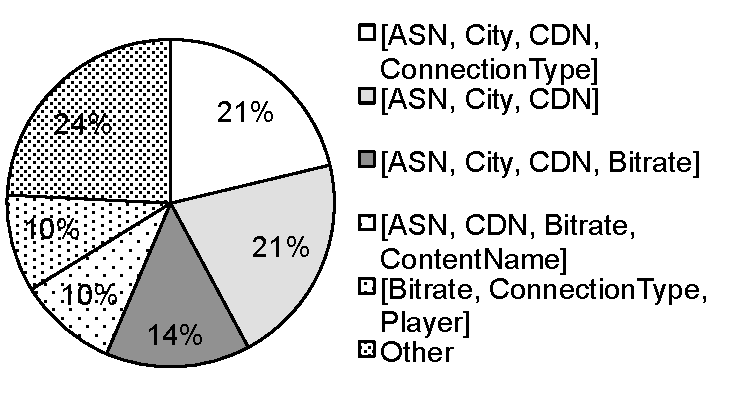
\includegraphics[width=.44\textwidth]{figures/cfa-insight-type-0.pdf}
        \label{subfig:insight-type-0}
}
%\hspace{-0.4cm}
\subfloat[AvgBitrate]
{
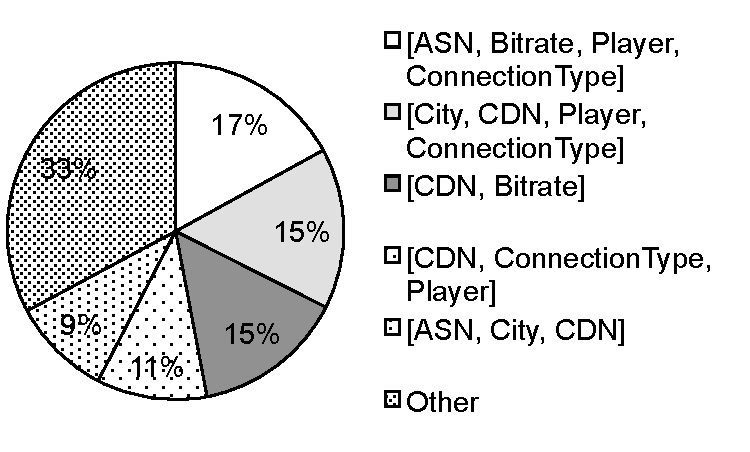
\includegraphics[width=.44\textwidth]{figures/cfa-insight-type-1.pdf}
        \label{subfig:insight-type-1}
}
%\hspace{-0.6cm}
\\
%\hspace{-1cm}
\subfloat[JoinTime]
{
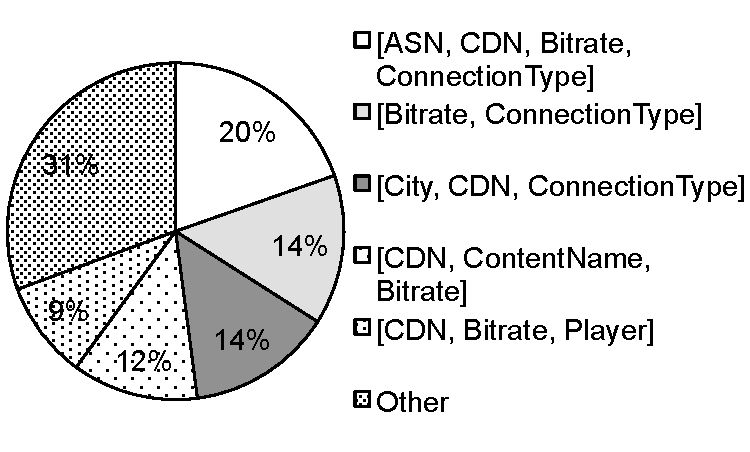
\includegraphics[width=.44\textwidth]{figures/cfa-insight-type-2.pdf}
        \label{subfig:insight-type-2}
}
%\hspace{-0.4cm}
\subfloat[VSF]
{
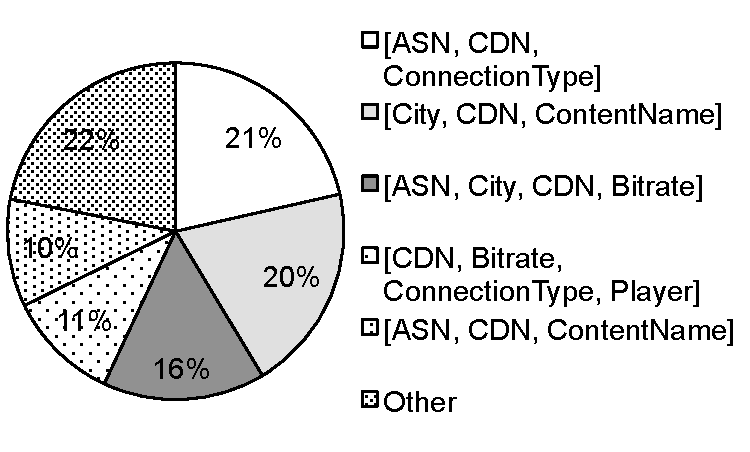
\includegraphics[width=.44\textwidth]{figures/cfa-insight-type-3.pdf}
        \label{subfig:insight-type-3}
}
%\hspace{-0.6cm}
%\vspace{-0.3cm}
\caption{Analyzing the types of critical features: This shows a 
breakdown of the total number of sessions assigned to a 
specific type of critical features.}
%\vspace{-0.3cm}
\label{fig:insight-type}
\end{figure}

We also see  interesting patterns unique to individual metrics.
\fCity is among the top critical features of BufRatio. This is perhaps because network
congestion usually depends on the volume of concurrent viewers in a specific
region.  \fBitrate (initial bitrate) has a larger impact on AvgBitrate than
on other metrics, since the videos in the dataset are mostly short content
(2-5 minutes) and AvgBitrate is correlated with initial bitrate. 
 Finally, \fContentName has a relatively large impact on failures (VSF) but not 
 other metrics, because VSF is sometimes due to the requested content not being ready. 

%Remember in \Section\ref{sec:insights} that there could be more critical

\myparatight{Distribution of types of critical features} 
%From the critical features that we learned, 
While the quality of about 50\% of sessions is impacted by
3-4 popular types of critical features, 15\% of sessions are
 impacted by a diverse set of more than 30 types of critical feature (not shown).  
This corroborates the need for expressive prediction models that handle the diverse
factors affecting quality (Section~\ref{subsec:expressive}). %\vyas{i cant parse this sentence}


\subsection{Values of Critical Features}
\label{subsec:insight-value}

%\comment
%{
%\myparatight{Real-world events revealed by critical feature values}
%We show that the real example of high dimensionality (\Section\ref{subsec:expressive}) can be revealed by values of critical features.
%%a confirmed one-day event when many Maryland Comcast users suffered from high VSF when accessing Level3.
%We find that 81\% of sessions using Comcast in Baltimore have $\fCDN=Level3$, $\fASN=7922$ (i.e., ``Comcast'') and $\fCity=Baltimore$ as values of critical features. 
%In contrast, only 17\% of other sessions (e.g., Verizon users in Maryland or Comcast users in California) have $CDN$, $ASN$ and $City$ as (part of) critical features. 
%%This shows that factors affecting video quality can be really reflected by the values of critical features.
%}

Next, we focus on the most prevalent {\em feature values} 
(e.g., a specific ASN or player).  
To this end, we define {\em prevalence} of a feature value  
by the fraction of video sessions matching this feature value 
that have this feature as one of their critical features; e.g., 
the fraction of video sessions from Boston that have \fCity
as one of their critical features.
If a feature value has a large prevalence, then the  quality 
of many  sessions that have this feature value can be 
explained by this feature.


%\myparatight{Most prevalent values of critical features}


%Note that the definition of prevalence is independent to the total population of sessions with a specific feature value (i.e., a small ISP can have a large prevalence if most of its sessions have its ASN as critical feature).
%In other words, what feature values have the highest impact on video quality if a session has it.

We present the values of critical features with a prevalence 
higher than 50\% for each quality metric and 
only consider a subset of the features ($ASN$, $City$, 
$ContentName$, $ConnectionType$) that appear 
prominently in  Figure~\ref{fig:insight-type}.  
We present this analysis with two caveats.  
First, due to proprietary concerns, we do not present 
the names of the entities, but focus on their characteristics.  
Second, we cannot confirm some of our hypothesis as it 
involves other  providers;  as such, we intend this result 
to be illustrative rather than conclusive. 

\begin{table}[t!]
%\begin{footnotesize}
\begin{tabular}{p{2.0cm}|p{3cm}|p{3cm}|p{3cm}|p{3cm}}
   &\textbf{$City$} & \textbf{$ASN$} & \textbf{$Player$} & \textbf{$ConnectionType$}\\ \hline \hline
BufRatio & Some major east-coast cities & & & Satellite, Mobile, Cable \\ \hline
AvgBitrate & & Cellular carriers & Players with different encodings & \\ \hline
JoinTime &  & Cellular carrier & & Satellite, DSL \\ \hline
VSF & & Small ISPs & & Satellite, Mobile \\
\end{tabular}
%\end{footnotesize}
%\vspace{-0.1cm}
\caption{Analysis of the most prevalent values of critical features. 
A empty cell implies that we found no interesting values in this combination.}
%\vspace{-0.2cm}
\label{tab:insight-popular-values}
\end{table}

Table~\ref{tab:insight-popular-values} presents some
anecdotal examples we observed.  
In terms of BufRatio, we see some of the major east 
coast cities (e.g., Boston, Baltimore) are more likely to be 
critical feature values than other smaller cities.  
We also see both poor (Satellite, Mobile) and broadband 
(Cable) connection types have high prevalence on 
BufRatio and JoinTime.  
This is because poor quality sessions are bottlenecked 
by poor connections, while some good quality sessions 
are explained by their broadband connections.  
``Player'' has a relatively large prevalence on AvgBitrate, 
because the content provider uses different  bitrate levels 
for different players (Flash or iOS).  
Finally, in terms of VSF, some small ISPs have large 
prevalence.  We speculate that this is because
their peering relationships with major CDNs are not 
provisioned, so their video sessions have relatively 
high failure rates.
%Cellular carriers have large impact on AvgBitrate and JoinTime, which are
%directly bottlenecked by available bandwidth.

%It is a bit surprising that there are also a few German cities (e.g., Berlin) and ISPs

